\section{实操:用结构体实现单链表}
\subsection*{什么是单链表?}
单链表是一种线性的数据结构\footnote{数据结构(Data structure),是一种组织、存储和管理数据的方式,它把一些数据通过某种特定的方式组织起来,以便于我们高效地访问和处理数据。}。它的数据存储方式是这样的:每个数据单元有两部分,其中一部分存储数据;而另一部分是一个指针,它指向下一个单元所在的位置。下一个单元也是两部分,其中一部分存储数据,而另一部分是一个指针,它指向下一个单元所在的位置。它和数组的区别在于,数组不需要单独的指针来存储下一个数据的位置,因为下一个位置就是取地址加一;而链表的各个单元可能分布于内存的各个区域,所以只有通指针才能找到下一数据的位置。图6.2展示了这种关系。\par
\begin{figure}[htbp]
    \centering
    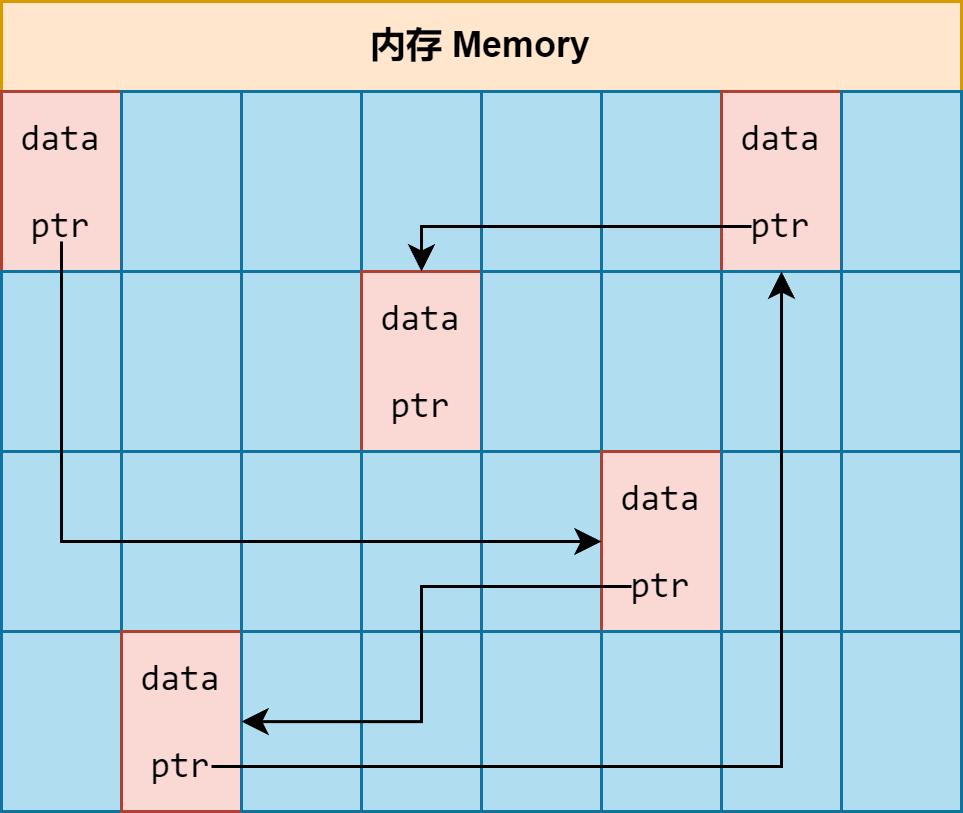
\includegraphics[width=0.6\textwidth]{../images/generalized_parts/06_list_in_the_memory_300.png}
    \caption{链表单元可以在内存中分散于各处}
\end{figure}
那么我们为什么要用链表而不是更容易实现的数组呢?这取决于我们的需求。在实际操作中,如果我们需要对一个数组的内容进行频繁的插入、删除操作,那么我们就需要在插入数据之前把对应位置之后的所有数据都向后挪一位;而如果要删除某个数据,我们就需要在删除数据之前把此位置之后的所有数据都向前递补。这是非常麻烦的。\par
\begin{figure}[htbp]
    \centering
    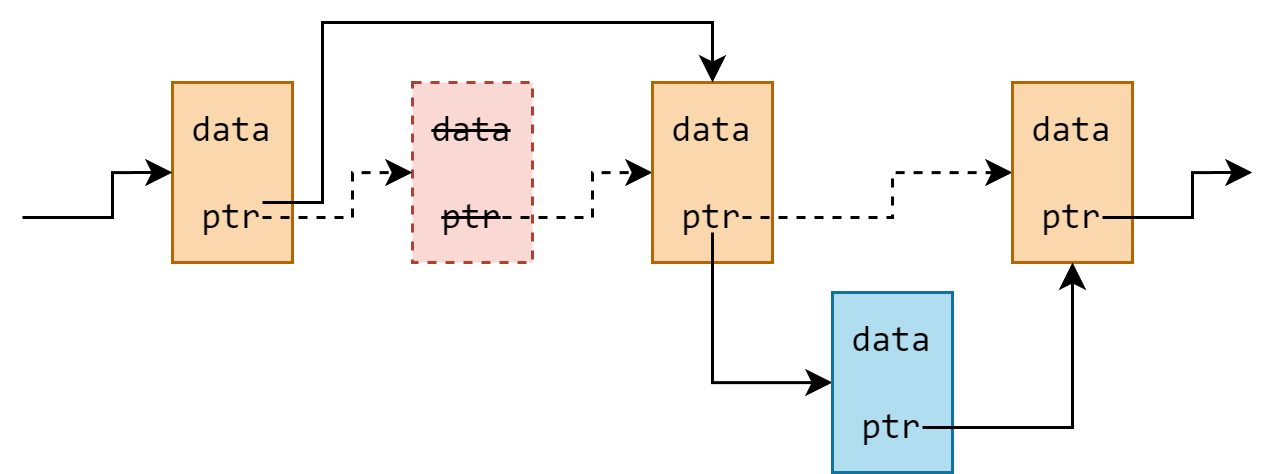
\includegraphics[width=\textwidth]{../images/generalized_parts/06_operation_on_list_300.png}
    \caption{链表的插入和删除操作}
    \footnotesize{蓝色的单元是待插入单元,红色的单元是待删除单元}
\end{figure}
而链表就能很高效地完成数据的插入和删除操作,如图6.3所示。如果要插入一个单元,那就把前一个指针指到新单元的位置上,并且让新指针指向下一个单元,于是插入操作就完成了。如果要删除一个单元呢,那就把前一个指针绕过本单元,直接指到后一个单元上,于是待删除的单元自然就可以抽身而去。\par
不止如此,单链表更大的优点在于可以方便地插入或删除一段数据,或者是把原链表中的一段转移到其它链表中。图6.4展示了片段转移的过程。无论这个片段有多长,我们都可以只通过两个起止点把待转移的片段摘下来,然后插入到另一个链表的某单元之后。\par
\begin{figure}[htbp]
    \centering
    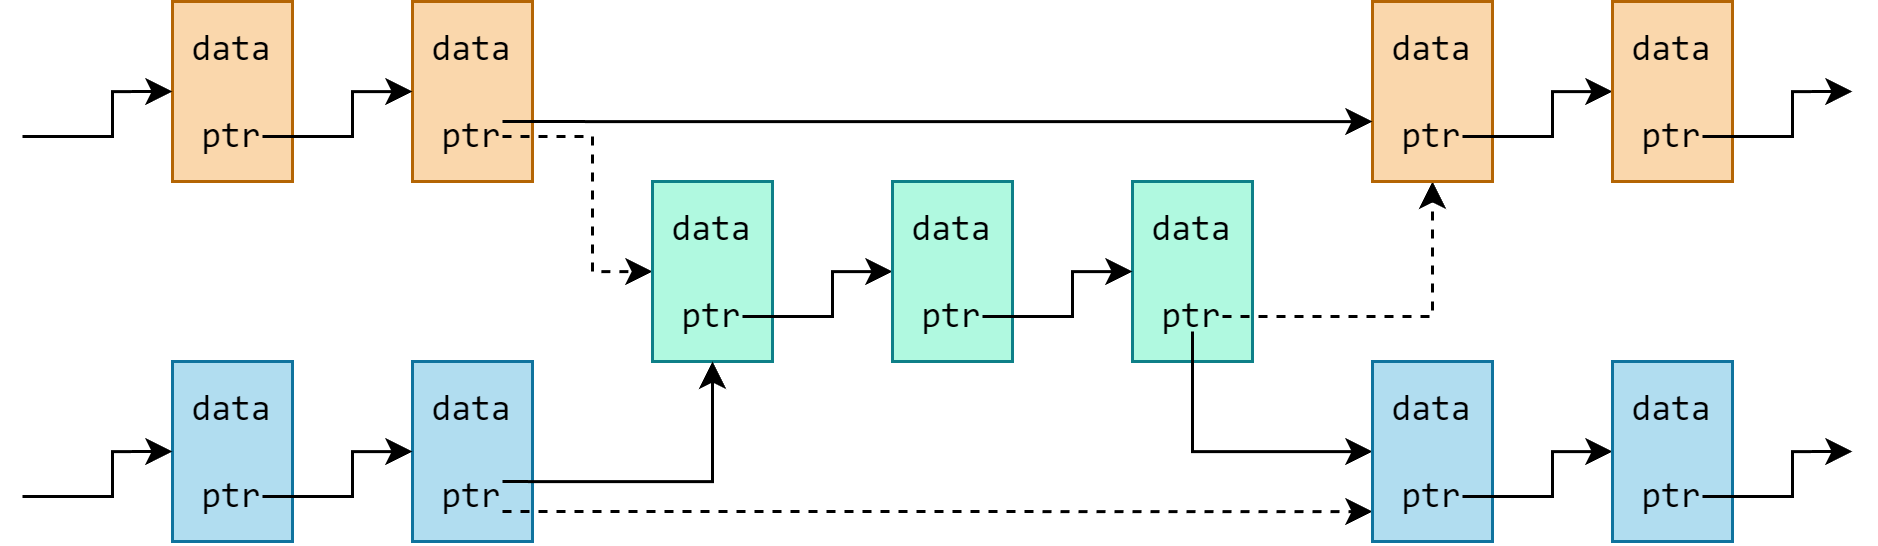
\includegraphics[width=\textwidth]{../images/generalized_parts/06_advanced_operation_on_list_300.png}
    \caption{链表的整段数据转移操作}
    \footnotesize{将绿色段从黄色链表中转移到蓝色链表中}
\end{figure}
那么了解了链表的基本概念之后,我们就可以试着自己来写一个链表,并配以相应的函数,来实现链表单元的插入、删除和整段转移操作。\par
\subsection*{链表的构建与内存回收}
链表的构建方式并不唯一,具本支持哪些功能也取决于我们的实际需求。在这里,出于教学目的,我们删繁就简,写一下链表的基本功能就行。\par
链表的每个单元都包含两部分——一个数据和一个指针,其中的指针要能指向某个单元。所以我们自然选择结构体的方式来实现它。
\begin{lstlisting}
struct Data {
    int num;
    Data *next;
};
\end{lstlisting}
我们可以定义一个不起存储作用的链表头 \lstinline@head@,它只负责指向本链表的第一条有效数据,比如这样:
\begin{lstlisting}
    Data head {0, nullptr}; //链表头,指向nullptr以免出现野指针
    head.next = new Data {5, nullptr}; //在链表末尾插入一个单元,用new分配
    (*head.next).next = new Data {8, nullptr}; // 再插入一个单元
\end{lstlisting}
这里的 \lstinline@head.next@ 就是指向第一个有效数据的指针。如果我们要指向第二个有效数据,我们就要先用 \lstinline@*@ 运算符取内容,然后再用成员访问运算符 \lstinline@.@ 找 \lstinline@next@。这样也太麻烦了。\par
C++为我们提供了更方便的方式,我们可以用指针的成员访问运算符 \lstinline@->@ 来直接通过指针访问对应的成员,而不必麻烦再取内容了。
\begin{lstlisting}
    head.next->next = new Data {8, nullptr};
    //head.next是一个指针,可以用指针的成员访问运算符直接得到它指向的next
    head.next->next->next = new Data {12, nullptr};
    //head.next->next同样是一个指针,我们还可以用->访问其内容
\end{lstlisting}\par
最后别忘记一个问题——我们是用 \lstinline@new@ 来添加新单元的,这也就意味着我们要用 \lstinline@delete@ 回收。但是我们不能直接 \lstinline@delete head.next@ 了事。这是因为,虽然 \lstinline@head.next@ 被回收了,但是它指向的那些内存地址还没有被回收。同时,因为 \lstinline@head.next@ 已经被回收了,所以我们也不能再通过 \lstinline@head.next->next@ 之类的语法来回收剩下的内存——也就是说,还有一个顺序的问题。\par
所以我们要考虑清楚怎么在建立一个单链表后妥善地回收动态内存,不然就会出现内存泄漏。正确的思路是,先回收链表末端的单元,再逐个向前依次回收,最后回收 \lstinline@head.next@。至于 \lstinline@head@,它本来就是静态的,我们不需要回收,作用域结束之后它自然就没了。\par
但是另一个棘手的问题在于,我们不知道末端的单元在哪里,所以要从 \lstinline@head.next@ 开始一个一个找,直到找到某个``\lstinline@next@ 指向 \lstinline@nullptr@''的单元为止。但是费了这么大劲才回收了一个单元,接下来我们还要再来这么好多轮,才能把所有单元都回收——这也太麻烦了。下面是这种思路的代码,它是一种最低效的方法,仅供读者了解。
\begin{lstlisting}
    while (head.next != nullptr) { //如果head之后的内容还末清空
        Data *p = head.next; //定义一个临时指针,准备从head.next开始向后寻找
        while (p->next->next != nullptr) { //说明*p->next还不是末尾单元
            p = p->next; //p向后移动一位
        }
        delete p->next; //现在*p->next就是最后一个单元,程序会回收这里的内存
        p->next = nullptr; //现在*p是最后一个单元
    }
\end{lstlisting}
这个方法既麻烦,又低效;而我们有更好的方法,一种是用删除的逻辑从头部开始清理,而另一种是用递归的方法从尾部开始清理。我们只讲第二种:
\begin{lstlisting}
void clear_list(Data *head) { //递归回收*head之后的所有动态内存
    if (head->next == nullptr) //如果*head之后没有动态内存
        return; //那就不需要回收什么了,直接return;结束本次调用
    clear_list(head->next); //先清理head->next之后的部分
    delete head->next; //再回收head.next
    head->next = nullptr;
    //现在head之后没有动态内存了,我们可以放心地把head->next置为nullptr
}
\end{lstlisting}\par
这个函数的设计目的是:任意给定一个头部单元指针 \lstinline@head@,回收 \lstinline@*head@(不含)之后的内存。\par
而它的递归思路是:每次调用时,先用 \lstinline@clear_list(head->next)@ 把 \lstinline@*head->next@(不含)之后的内存回收,然后回收 \lstinline@*head->next@。\par
\begin{figure}[htbp]
    \centering
    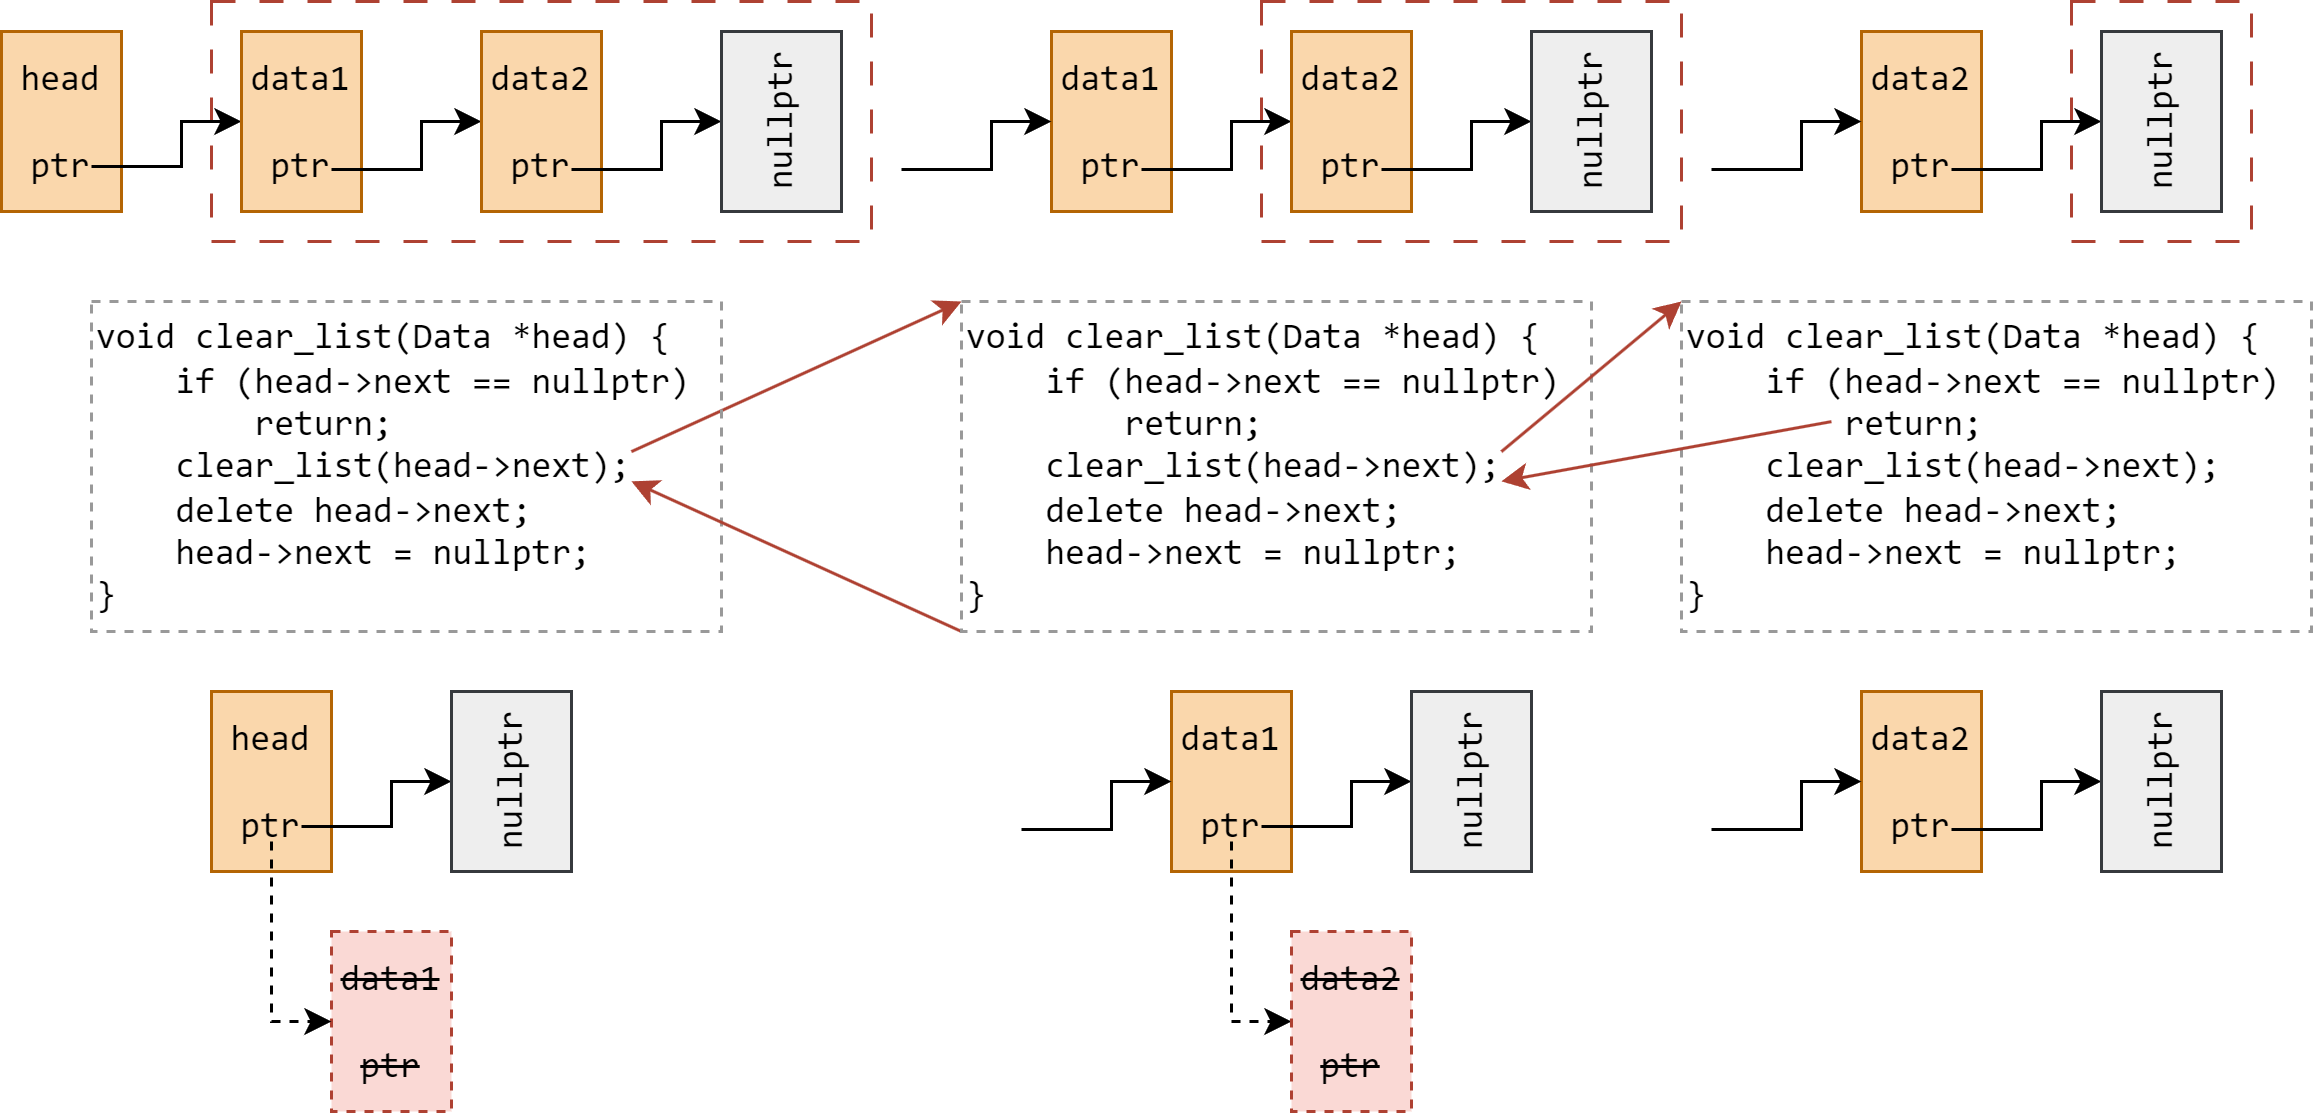
\includegraphics[width=\textwidth]{../images/generalized_parts/06_process_of_clear_list_300.png}
    \caption{递归回收链表的过程示意图}
\end{figure}
\subsection*{链表的基础功能}
接下来我们考虑对单个单元进行插入和删除操作。为了简化,我们规定:插入操作只能插入到指定单元的下一位,而删除操作只能删除指定单元的下一个单元。这些操作都很简单,但是你需要非常小心——尤其是在语句的顺序安排方面。\par
我们先来看插入操作。这个操作的具体过程可以分为三步,见图6.6及代码中注释。\par
\begin{lstlisting}
void insert_after(Data *head, int n) { //在*head下一位置插入n
    Data* p = { new Data{n,nullptr} }; // 分配动态内存,并初始化其num成员
    p->next = head->next; //插入数据的下一位指向当前的*head->next
    head->next = p; //head->next指向*p,注意顺序不要颠倒!
}
\end{lstlisting}
\begin{figure}[htbp]
    \centering
    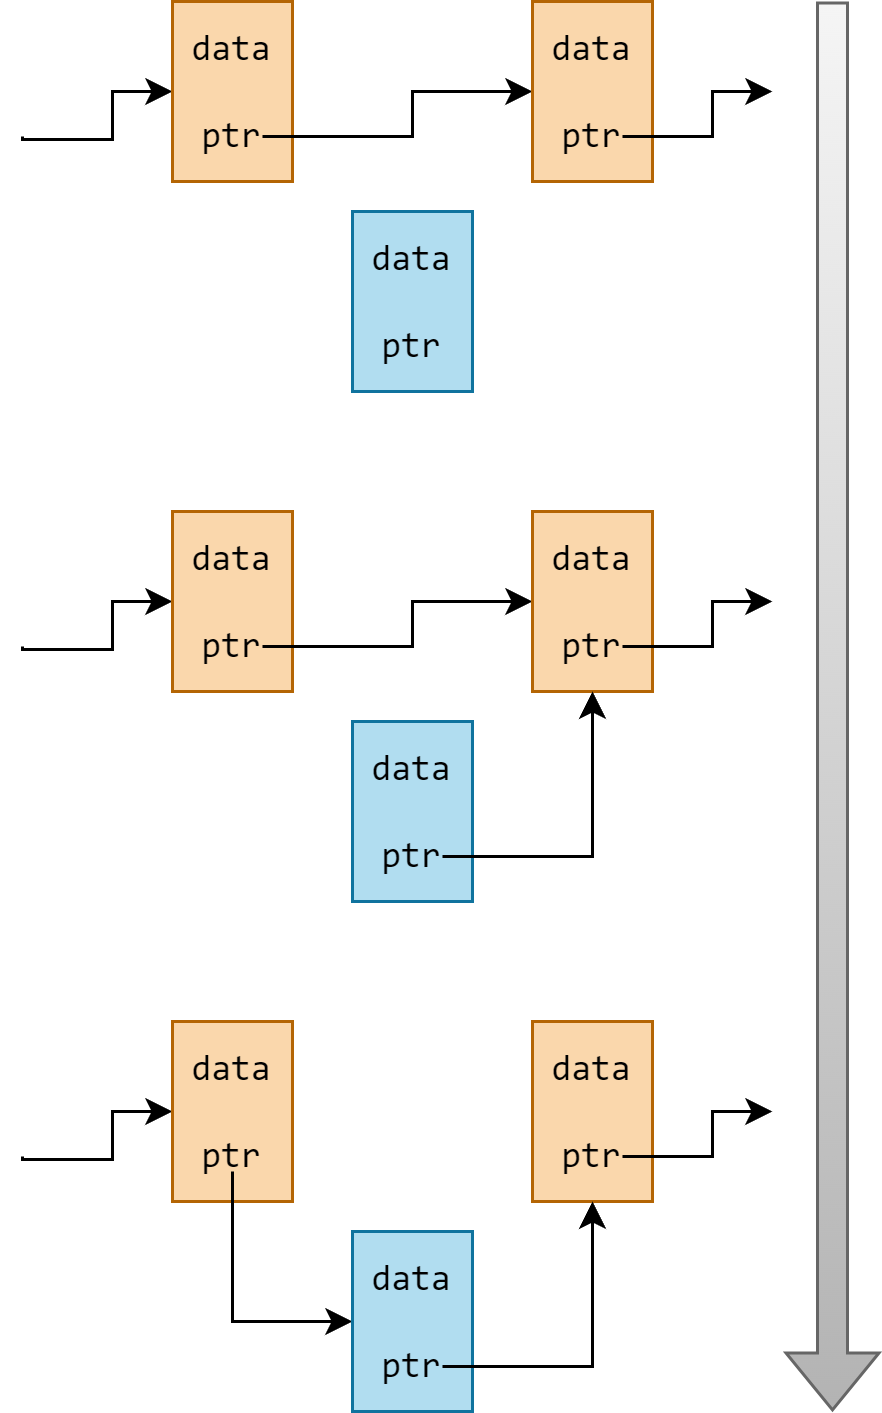
\includegraphics[width=0.4\textwidth]{../images/generalized_parts/06_insertion_into_a_list_300.png}
    \caption{插入数据的过程}
\end{figure}\par
读者一定要注意这些操作的顺序安排。如果我把 \lstinline@head->next=p@ 放在前面,那就会出现一个问题,\lstinline@head->next@ 赋值之后,它原本所指向的单元就找不到了。\par
当你熟悉了语法之后还可以把这三步简化成一步:
\begin{lstlisting}
void insert_after(Data *head, int n) { //在*head下一位置插入n
    head->next = new Data{n,head->next}; //三步并作一步
}
\end{lstlisting}
再来看删除操作,我们需要写一个函数,给定某个 \lstinline@Data *head@,这个函数能删除它后面的一个单元。这个操作的过程可以分为两步,见图6.7及代码中注释。
\begin{lstlisting}
bool delete_after(Data *head) {
//删除*head下一位置的数据,并返回true;若*head是末尾元素,删除失败,返回false
    if (head->next == nullptr) //说明*head就是末尾元素
        return false;  //*head是末尾元素,无法再删除后面内容
    //这里应当用else块,不过也可以省掉
    //因为if块内会直接return,所以后面的代码肯定是在条件为false情况下运行的
    Data *p = head->next; //临时指针p指向*head->next
    head->next = p->next; //head->next指向更后一个元素
    delete p; //回收p指向的内存
    return true;
}
\end{lstlisting}
\begin{figure}[htbp]
    \centering
    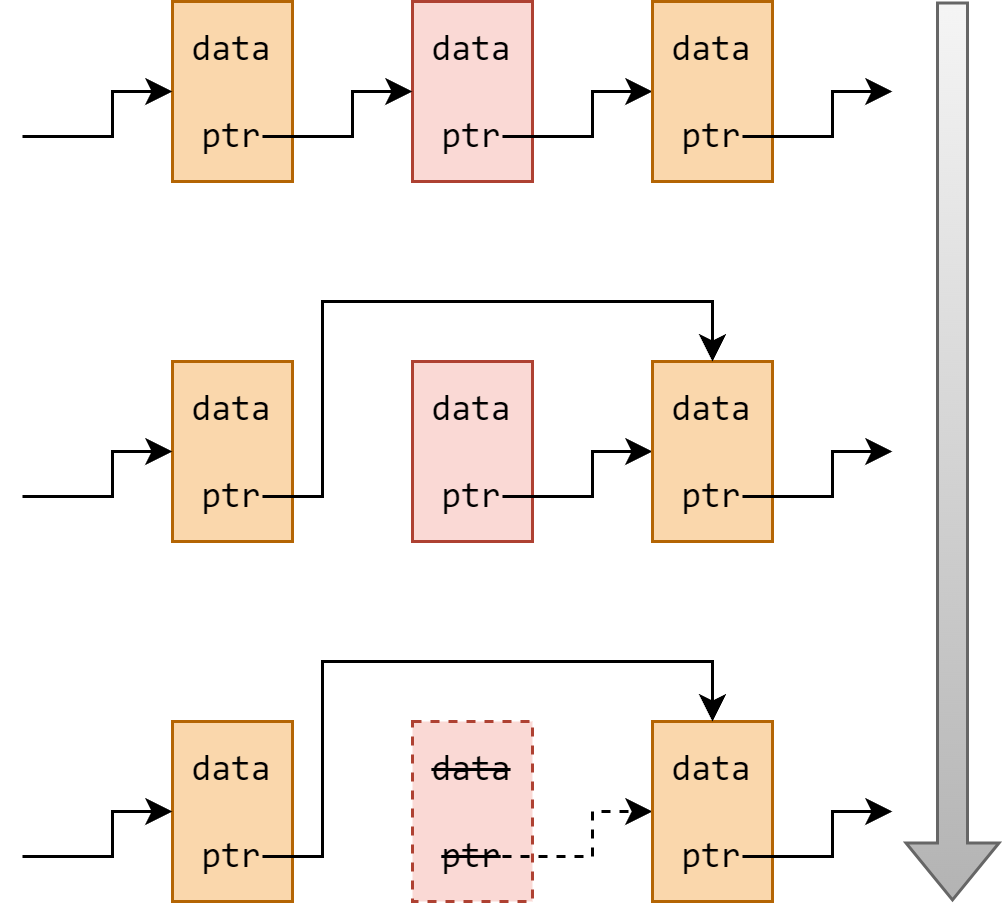
\includegraphics[width=0.45\textwidth]{../images/generalized_parts/06_deletion_operation_on_a_list_300.png}
    \caption{删除数据的过程}
\end{figure}\par
这里指得一提的是返回值。按理说删除操作只是 \lstinline@delete_after@ 函数的副作用,不需要求值。但是有些情况下我们可能需要根据返回值的实际情况来调整其它值。例如,我可能有另外一个值用来记录这个单链表的长度,那么返回值就决定了我们要不要在删除操作之后让这个长度减一。
\begin{lstlisting}
    if (delete_after(ptr)) { //如果删除成功
        --size; //size自减
    }
    //否则size不变,什么也不做
\end{lstlisting}\par
\subsection*{链表的进阶功能}
接下来我们可以来试着实现一些链表的进阶功能:片段插入、片段删除和片段转移。其中的片段插入可以用片段转移的方式来实现,所以我们只需要关注后两个就行。我们先来看片段删除操作。\par
我们在这里要写一个函数,删除从某个单元(不包含)开始到某个单元(包含)为止。\footnote{关于``是否包含两端''的问题,其实有很多种写法,都可以实现。在此处我们选择使用此套方案,即左端不包含而右端包含。}
\begin{lstlisting}
bool delete_after(Data *head, Data *tail) {
//删除*head之后(不包含)直到*tail为止(包含)的单元。若删除失败,返回false
    if (head == tail) //说明没有任何数据需要清理
        return false; //删除失败
    if (tail == nullptr) { //说明我们需要删除*head之后的所有内容
        clear_list(head); //当然是用clear_list啦
        return true; //删除成功
    }
    Data tmp_head {*head}; //用*head来直接为tmp_head初始化
    head->next = tail->next; //绕过待删除段,直接指向*tail->next
    tail->next = nullptr; //tail指向nullptr,现在待删除片段就被剥离出来了
    clear_list(&tmp_head); //以tmp_head为头,清理这段链表
    return true; //删除成功
}
\end{lstlisting}
这段代码对于初学者来说可能有点复杂,所以看不懂也没关系。如果还可以勉强看懂一部分,那不妨再看一看下面的讲解:\par
这里的 \lstinline@delete_after@ 是一个重载函数,它既有 \lstinline@(Data*)@ 版本,又有 \lstinline@(Data*,Data*)@ 版本。当传入单个指针时,就意味着删除一个单元;当传入两个指针时,就意味着删除一串单元。这种重载思路在STL中比较常用。\par
在函数体部分,我们需要判断一种非法情况,也就是 \lstinline@head==tail@。在这种情况下,\lstinline@head@ 到 \lstinline@tail@ 之间的片段是空,所以这种操作没有意义。\par
那么在 \lstinline@tail==nullptr@ 的情况下,我们可以直接删除从 \lstinline@head@(不包含)开始的所有单元。这样的话,最佳选择就是直接使用内存回收函数 \lstinline@clear_list@ 解决问题。\par
现在我们再来考虑一般的情况——\lstinline@head@ 和 \lstinline@tail@ 都是这个链表中的单元。\footnote{实际的情况远比这个复杂,比如说 \lstinline@head==nullptr@ 的时候怎么处理;\lstinline@head@ 和 \lstinline@tail@ 不在同一链表中的情况怎么处理,诸如此类。不过我们在这里只是用代码来进行演示和学习,不需要像实际工程中那样做得面面俱到。那太复杂了。}我们的思路是把这个片段给剥离出来,变成一个单独的临时链表,然后用 \lstinline@clear_list@ 直接清理这个单独的链表,如图6.8所示。\par
\begin{figure}[htbp]
    \centering
    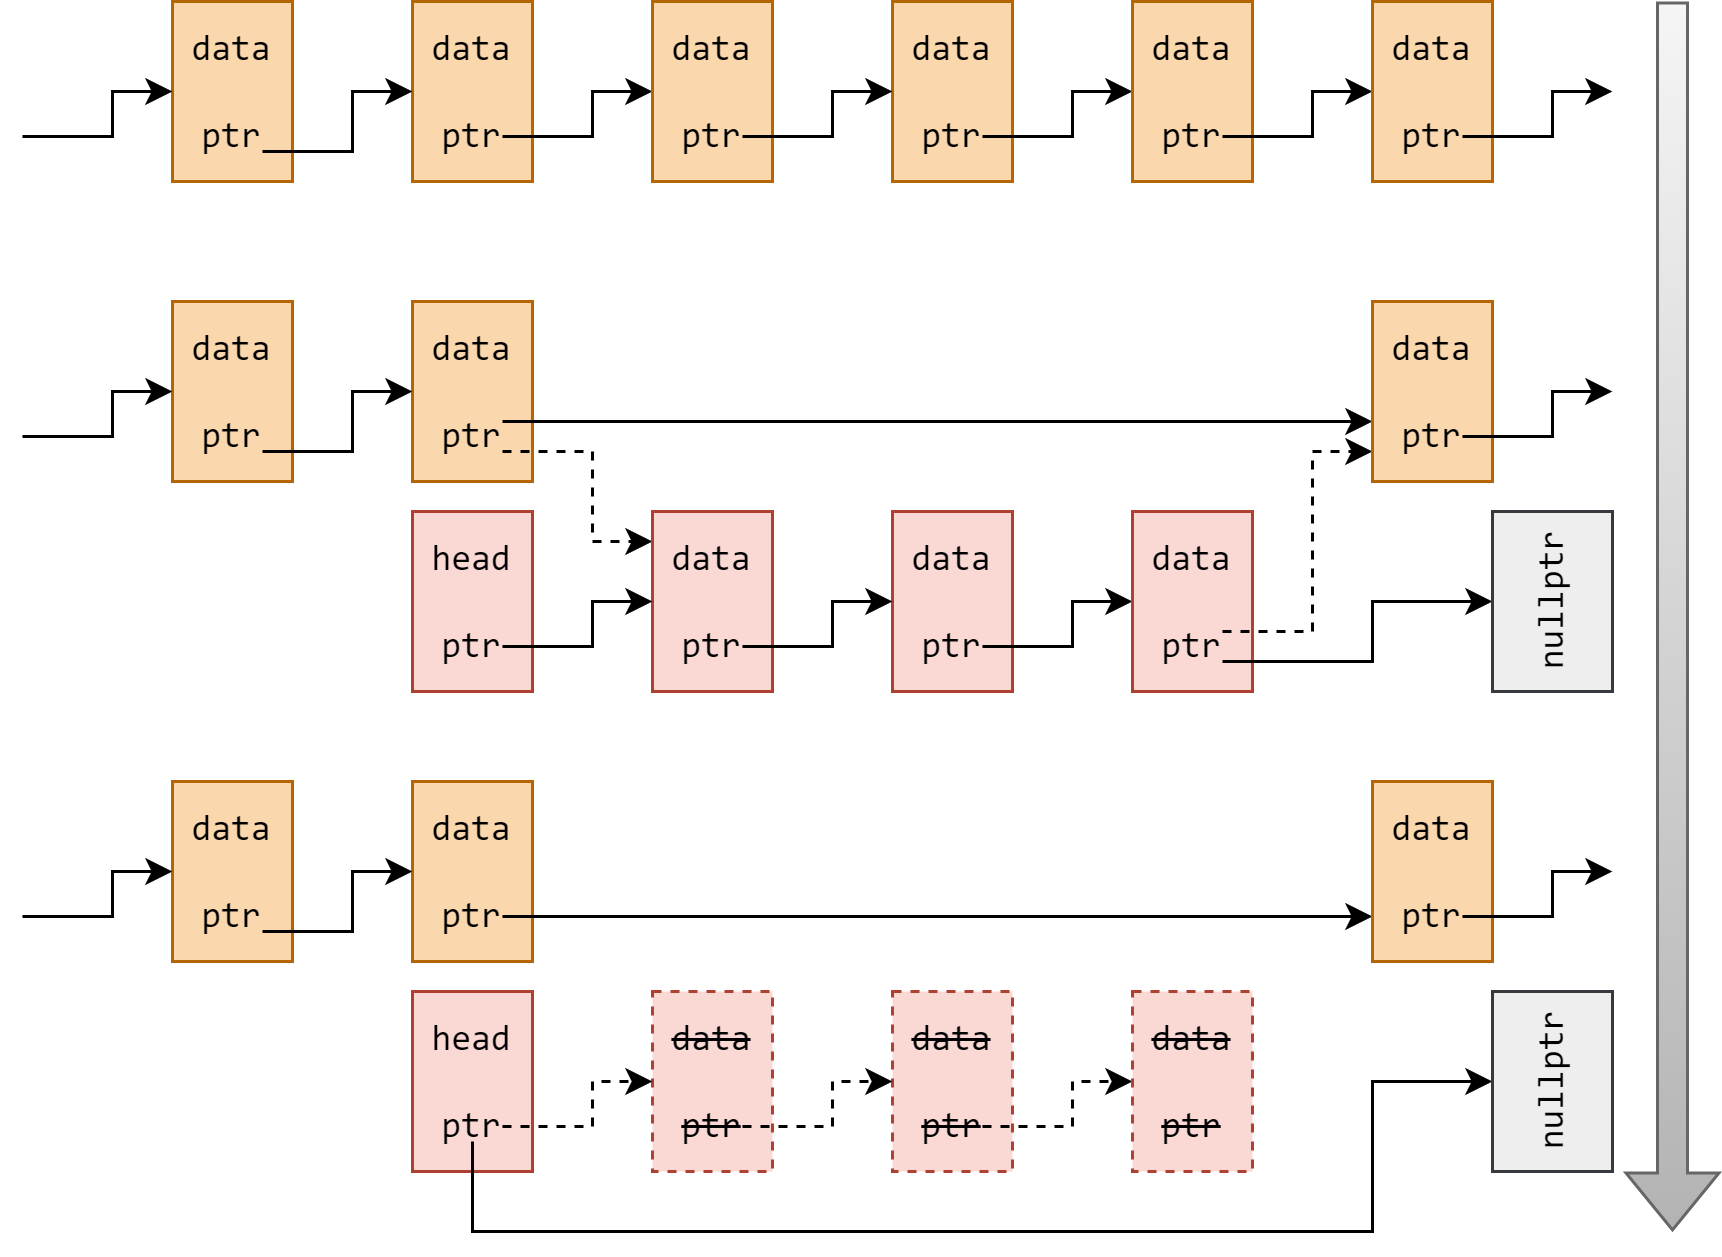
\includegraphics[width=0.9\textwidth]{../images/generalized_parts/06_range_deletion_operation_on_a_list_300.png}
    \caption{链表的片段删除操作}
\end{figure}
在剥离操作中,我们定义了一个临时的链表头 \lstinline@tmp_head@,并且用 \lstinline@*head@ 来初始化它\footnote{在后面我们会讲到,这里用到了默认拷贝构造函数。},这样 \lstinline@tmp_head@ 和 \lstinline@*head@ 就有了相同的值,只是它们地址不同。我们就打算把待删除的片段转移到以 \lstinline@tmp_head@ 为首的链表中。\par
在剥离的过程中我们也要注意顺序,否则就容易把信息搞丢:第一步,我们把原链表缝起来,这时 \lstinline@tmp_head@ 还能连到待删除段,并且 \lstinline@tail@ 也能找到需要缝起来的部分,所以一切安然无恙;第二步,我们把 \lstinline@tail@ 段也拆下来,这样就彻底断绝了两个链表的联系。\par
剥离完成之后我们直接清理 \lstinline@tmp_head@ 链表的动态内存就行,这里很简单。\par
那么我们再来看链表片段转移的操作。一个片段转移函数——我们起名 \lstinline@transfer@,它应该有三个参数:前两个参数描述这个片段从哪里到哪里,后一个参数描述这个片段要转移到何方(目的地)。\par
读者可以延续我们刚才的思路,并参考图6.4的示意来自行完成这个函数。而这里我们选择另一种写法:
\begin{lstlisting}
void transfer(Data *head, Data *tail, Data *dest) {
//片段转移,把*head之后(不包含)直到*tail为止(包含)的单元移到*dest之后
    if (head == tail || dest == nullptr) //这两种情况下转移没有意义
        return;
    if (tail == nullptr) { //这种情况不方便我们处理,我们把tail改成指向末尾单元
        for (tail = head; tail->next != nullptr; tail = tail->next) {
            ; //for循环的逻辑是,从head开始找,直到tail->next==nullptr为止
        }
        if (head == tail) //仍需当心head==tail的可能
            return;
    }
    swap(tail->next, dest->next); //swap函数需要utility或string_view库
    swap(head->next, dest->next); //是一种技巧,读者不必强求掌握
}
\end{lstlisting}
这里再说明两点:\par
其一,在这里 \lstinline@tail==nullptr@ 的情况下我们要处理是比较麻烦的,因为当后面涉及到 \lstinline@tail->next@ 的时候我们必须得让 \lstinline@tail@ 有意义才行——\lstinline@nullptr@ 肯定不行。所以为了解决这个问题,我们要把 \lstinline@tail@ 改成指向末尾单元。怎么做呢?只能从 \lstinline@head@ 开始一个个找,直到找到一个``\lstinline@tail->next==nullptr@''的情况,这时 \lstinline@tail@ 就是我们想找的末尾单元了。\par
我们可以用循环结构来找,本段代码就是这样操作的。除此之外还可以递归,参照这段代码来找也行:
\begin{lstlisting}
Data* find_tail(Data* head) { //从head开始找
    if (head->next == nullptr) //如果head->next==nullptr
        return head; //那么它就是我们要找的tail
    return find_tail(head->next); //否则就从head->next开始找
}
\end{lstlisting}\par
其二,这里转移操作的写法很独特(也很简洁,不是吗)。这里用文字很难讲清楚,读者可以直接看图6.9,很直观。在这里我们用标准库中的 \lstinline@swap@ 函数,它可以交换两个指针的值\footnote{实际上 \lstinline@swap@ 是一个函数模板,当我们尝试使用它时,程序会生成一个关于 \lstinline@Data*@ 类型的实例。我们会在第十一章中介绍相关的知识。},也就相当于交换它们的指向。于是我们可以通过先交换 \lstinline@tail->next@ 和 \lstinline@dest->next@,再交换 \lstinline@head->next@ 和 \lstinline@dest->next@ 的方式来实现这个功能。\par
\begin{figure}
    \centering
    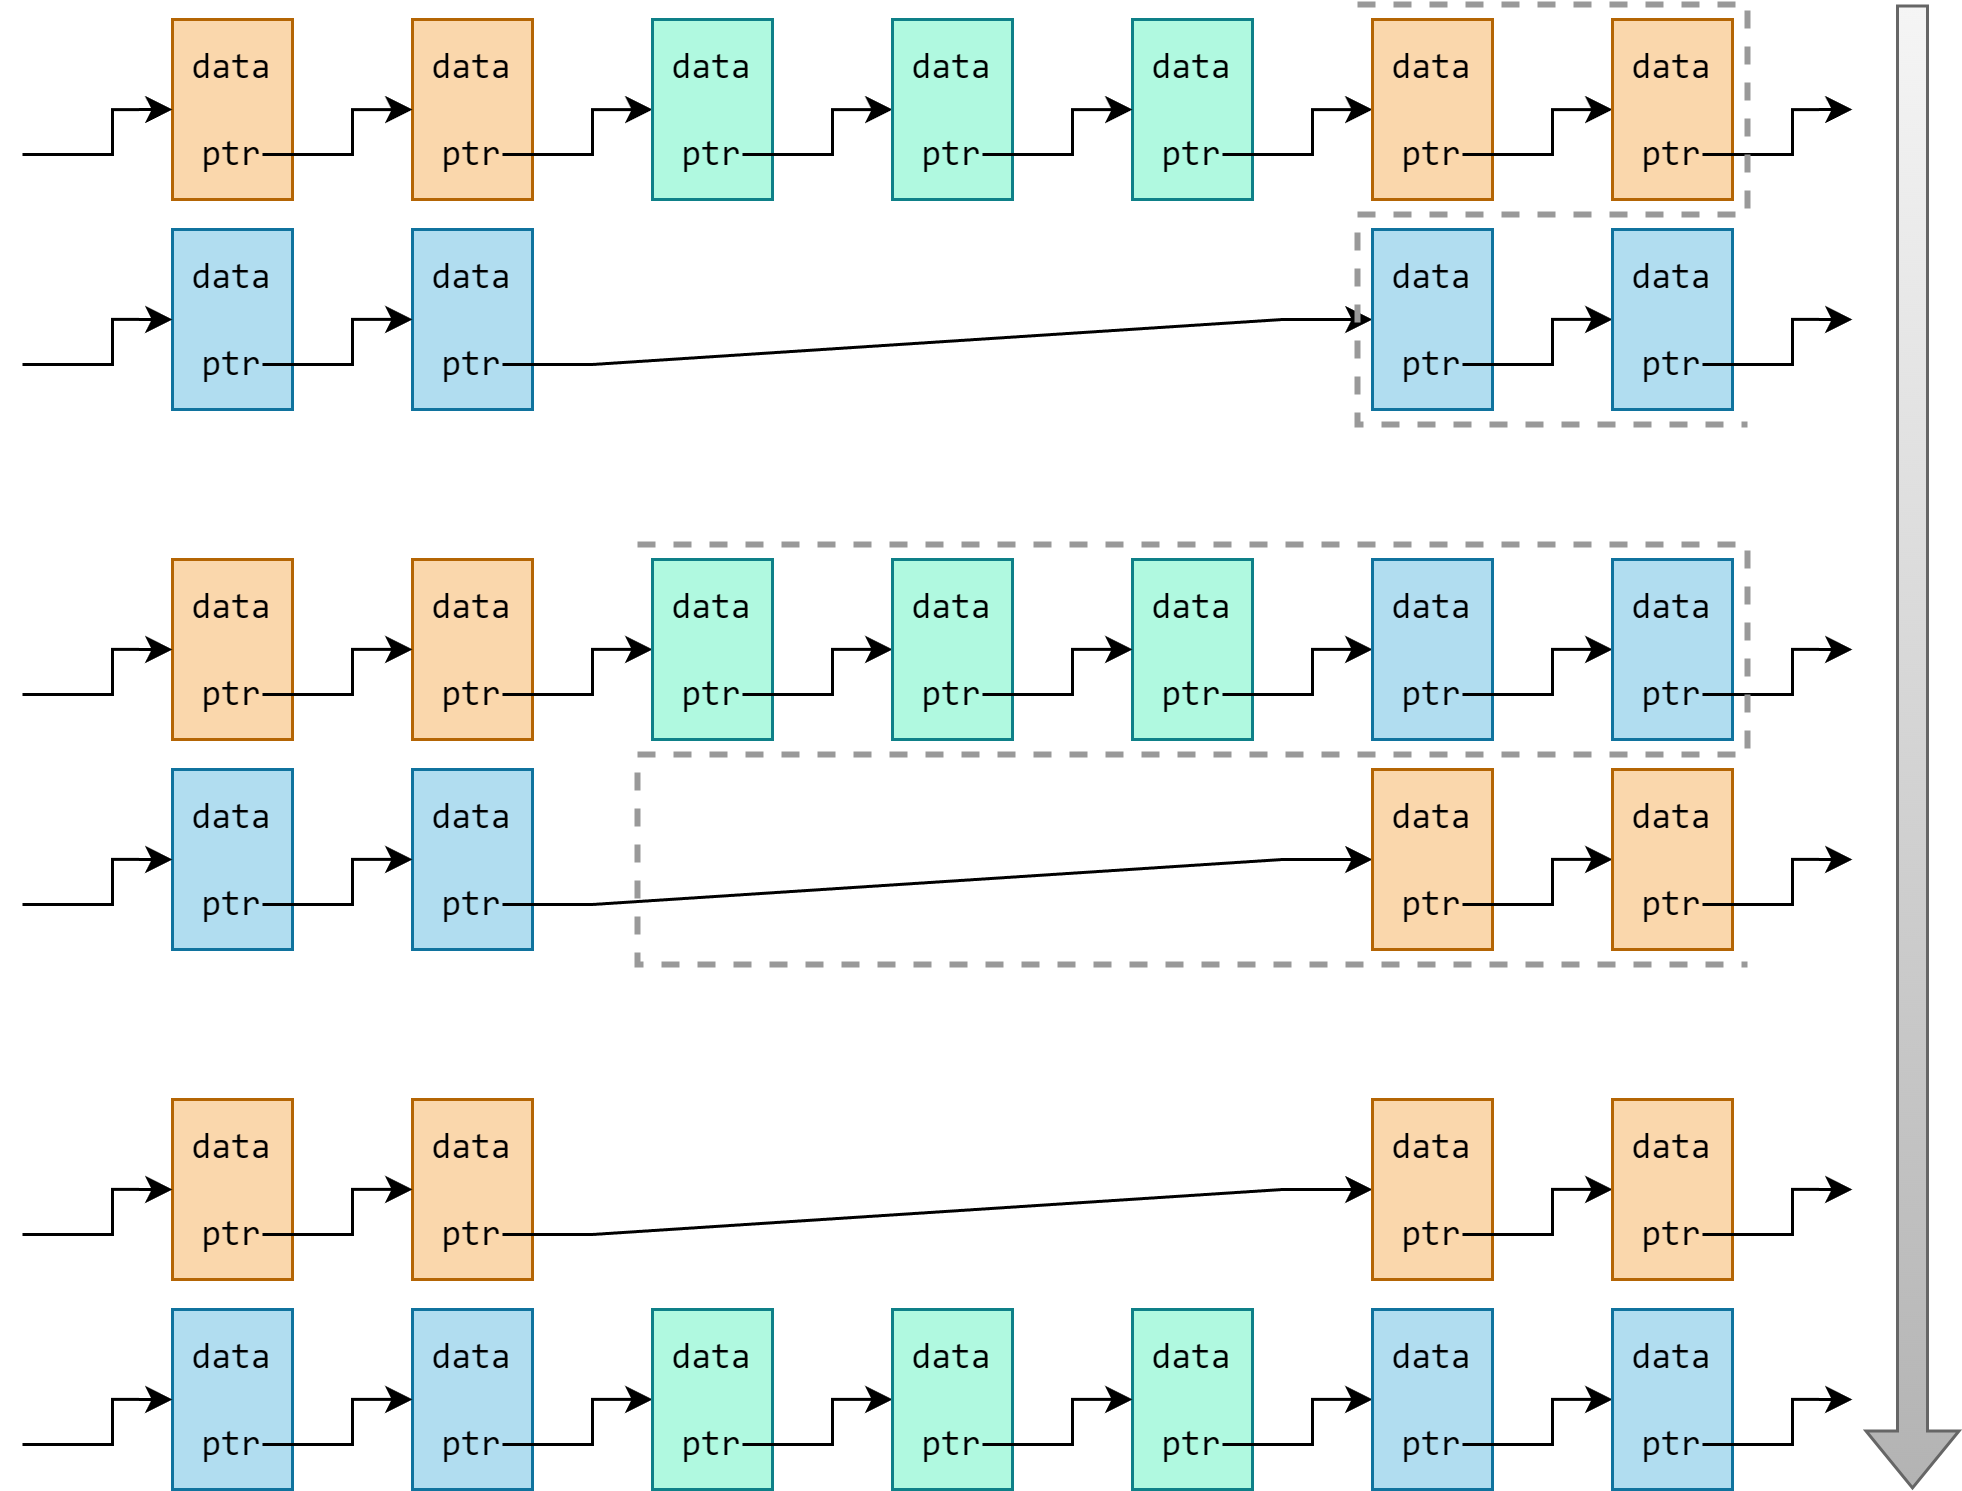
\includegraphics[width=\textwidth]{../images/generalized_parts/06_range_transfer_between_lists_300.png}
    \caption{片段转移操作的示意图}
\end{figure}
